\chapter{Présentation du sujet}
Aboard Engineering étant une entreprise spécialisée dans les domaines de
l'informatique embarquée, les problématiques logicielles qu'elle rencontre sont
liées au matériel sur lequel sera déployé le code développé. Pour facilité ce
type de développement, les concepteurs de logiciels embarqués se tournent de
plus en plus vers des outils de \gloss{mbd} qui permet d'utiliser des langages
de haut niveau -- souvent graphiques -- pour la conception et la spécification
des systèmes à développer. On peut citer par exemple Matlab\up{\circledR}
Simulink\up{\circledR} qui est un outil permettant de définir graphiquement sous
forme de schéma logique le fonctionnement de systèmes complexes. C'est
d'ailleurs l'outil utilisé par Aboard Engineering pour définir ses fonctions de
contrôle moteur. Les avantages des ces modèles sont multiples. Premièrement, les
outils de \gloss{mbd} permettent de simuler l'exécution du système afin de
vérifier son fonctionnement. Ensuite, ces outils embarquent généralement un
générateur de code afin de générer le code correspondant à ces modèles,
allégeant grandement le travail des concepteurs et évitant au maximum les
erreurs faites lors de développement \og manuel\fg{}. En reprenant l'exemple de
Matlab\up{\circledR} Simulink\up{\circledR}, la suite intègre un générateur de
code embarqué temps réel appelé \gloss{rtw}. Il génère aujourd'hui le code des
prototypes de fonctions de contrôle moteur développés par l'équipe. J'y
reviendrai dans la section \ref{sec:rtw} plus en détail.

Comme dit précédemment, la génération de code facilite le travail de conception
et de réalisation de prototype. Cependant, pour pouvoir compiler le code de
plusieurs modules différents en une seule application, il reste des étapes à
réaliser. C'est ici que la plateforme de prototypage rapide \gloss{orianne}
entre en jeu. C'est son rôle de mettre en relation ces modules et de créer la
\og glue \fg{} entre tous les composants.\\
\Gloss{orianne} est composée de plusieurs parties que nous appellerons \og
composants \fg{}. Je détaillerai les composants présents lors de mon arrivée
ainsi que ceux sur lesquelq j'ai travaillé dans la section \ref{sec:rtw}.

\section{La génération de code embarqué (Matlab\up{\circledR} \gloss{rtw} vs.
\gloss{qgen})}
\subsection{État des lieux}
Le développement d'une application pour un calculateur moteur n'est pas une
mince affaire. De nombreux modèles sont nécessaire à la spécification de tous
les aspects du fonctionnement d'un moteur ou des différents commandes
utilisateur (pédales, boîte de vitesse, etc.) par exemple. À cela peut s'ajouter
le gestion d'une configuration hybride -- un moteur thermique couplé à un moteur
électrique -- nécessitant une gestion plus pointue de l'énergie.

Une fois complets, ces modèles ont vocation à être traduit en code source qui
sera compilé puis intégré dans un calculateur. C'est donc ce code compilé qui
est la base du fonctionnement d'un véhicule. On comprend alors les contraintes
de fiabilité et de performance sous-jacentes.\\

Pour générer ce code, nous utilisons Matlab\up{\circledR} \gloss{rtw}. C'est un
générateur de code embarqué temps réel puissant et reconnu pour fournir du code
suivant les normes en vigueur dans l'automobile.
Le code généré conttient toute la logique métier et donc l'essentiel de la
complexité de l'application. Sur ce point, Matlab\up{\circledR} \gloss{rtw}
fournit des résultats très bons en terme de temps d'execution, de mémoire
utilisée ou de taille de pile lors des appels aux fonctions des modules.\\

Cependant, une ombre plane sur ce tableau. La suite Matlab\up{\circledR} coûte
très cher. Même pour une entreprise -- d'autant plus pour une entreprise de
petite taille comme Aboard Engineering --, les coût des licences
Matlab\up{\circledR} couvrant toute la suite nécessaire à l'ensemble du
processus de production n'est pas négligeable et compte pour beaucoup dans les
charges liées à un projet.\\

La problématique est alors de retrouver les même garanties de performance et de
qualité du code produit par Matlab\up{\circledR} sans le coût exorbitant
qu'engendre l'achat de licences. C'est pourquoi Aboard Enginnering a décidé de
se tourner vers une alternative libre : \gloss{qgen} et \gloss{projectp}.

\subsection{\gloss{qgen}}
A la base de \gloss{qgen}, on trouve un projet open source appelé
\gloss{projectp}. Le but du projet P est de supporter le \gloss{mbd} pour des
système temps réel embarqués en fournissant un framework de generation de code
open source capable de :
\begin{enumerate}
  \item vérifier l'intégrité d'un point de vue sémantique de sèstème conçus avec
	différents langages de modélisation (Matlab\up{\circledR}
	Simuling\up{\circledR}, Scicos, Xcos, SysML, MARTE, UML) ;
  \item générer du code source optimizé pour des langages de programmation
	(Ada, C/C++) et des alngages de synthèse (VHDL, SystemC) ;
  \item supporter des processus de certification de différents domaines
	(avionique, spacial, automobile).
\end{enumerate}

\begin{figure}[h]
  \centering
  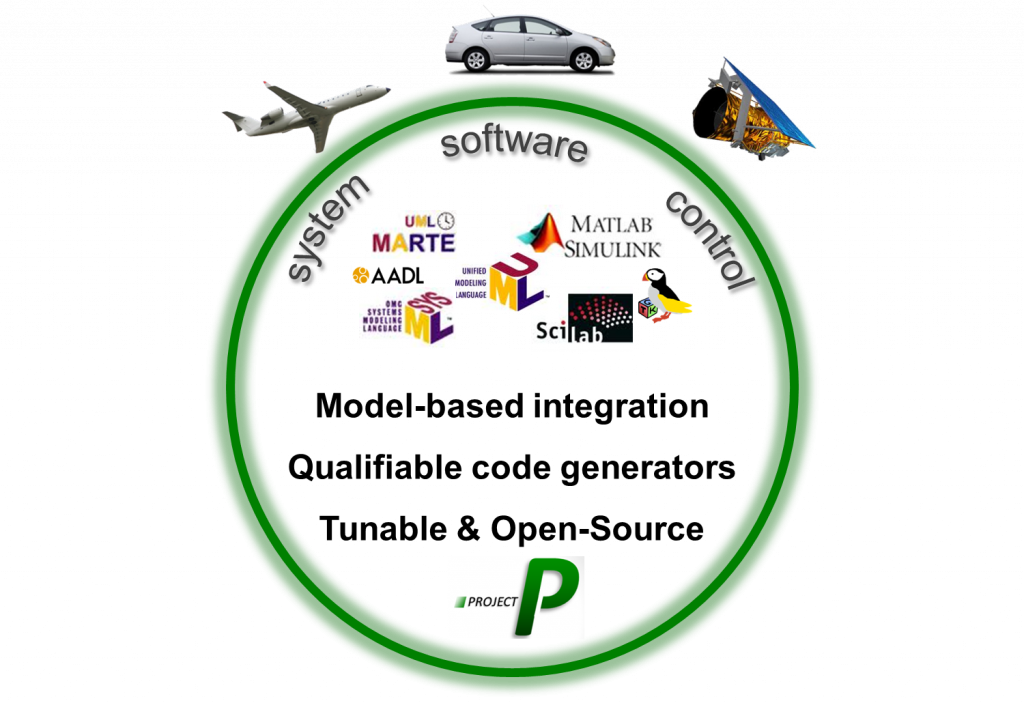
\includegraphics[scale=0.3]{images/projectp}
  \caption{Project P -- Source : {\tt http://www.open-do.org/projects/p/}}
  \label{fig:projectp}
\end{figure}

Parmis les collaborateurs à ce projet, on trouve des grands groupes industriels
(Airbus, Astrium, Continental, Rockwell Collins, Safran, Thales) des PME
(AdaCore, Altair, Scilab Enterprise, STI), des sociétés de services (ACG, Aboard
Engineering, Atos Origins) mais aussi des centres de recherche (CNRS, ENPC,
INRIA, ONERA).\\

À partir de ça, AdaCore a développé un produit commercial à partir des
technologies développées dans \gloss{projectp} : \gloss{qgen}.

\begin{figure}[h]
  \centering
  
\includegraphics[scale=0.2]{images/qgen}
  \caption{QGen -- Source AdaCore}
  \label{fig:qgen}
\end{figure}

\section{Les outils de la plateforme}
\lipsum
